\documentclass{svproc}
%
\usepackage{graphicx}%
\usepackage{multirow}%
\usepackage{amsmath,amssymb,amsfonts}%
\usepackage{mathrsfs}%
\usepackage[title]{appendix}%
\usepackage{xcolor}%
\usepackage{textcomp}%
\usepackage{manyfoot}%
\usepackage{booktabs}%
\usepackage{algorithm}%
\usepackage{algorithmicx}%
\usepackage{algpseudocode}%
\usepackage{listings}%
\usepackage{url}
\def\UrlFont{\rmfamily}

\renewcommand{\topfraction}{.99}
\renewcommand{\dbltopfraction}{.99}
\renewcommand{\bottomfraction}{.99}
\renewcommand{\textfraction}{.01}
\renewcommand{\floatpagefraction}{0.9}
\renewcommand{\dblfloatpagefraction}{0.9}

\usepackage[normalem]{ulem}
\usepackage{bm}
\usepackage{xspace}
\usepackage{subcaption}

\usepackage{color}
\def\green#1{\textcolor[rgb]{0,0.6,0}{#1}}
\def\black#1{\textcolor[rgb]{0,0,0}{#1}}
\def\dgreen#1{\textcolor[rgb]{0.02,0.50,0.05}{#1}}
\def\gray#1{\textcolor[rgb]{0.5,0.5,0.7}{#1}}
\def\red#1{\textcolor{red}{#1}}
\def\blue#1{\textcolor{blue}{#1}}
\def\Blue{\color[rgb]{0,0,1}}
\def\Red{\color[rgb]{1,0,0}}
\def\Dgreen{\color[rgb]{0.02,0.55,0.04}}
\def\Black{\color[rgb]{0,0,0}}
\def\ignore#1{}

\usepackage[normalem]{ulem}
\usepackage{bm}
\usepackage{booktabs}
\usepackage{xspace}
\usepackage{subcaption}

% track-changes helpers (kept from last year's setup)
\newcommand{\add}[1]{\textcolor{blue}{#1}}
\newcommand{\erase}[1]{\textcolor{red}{\sout{#1}}}
\def\subst#1#2{\add{#1}{ \erase{#2}}}

% parameters definition (same convention as docs/journal.tex)
\def\post{\rho}                 % posting probability
\def\BoundedConfidence{\epsilon} % bounded confidence (rejection) threshold
\def\feed{F}                    % feed
\def\Stubbornness{\mu}           % stubbornness
\def\maxfollower{S_{\it fol}}    % max followee capacity
\def\maxfeed{S_{\it fd}}         % feed capacity
\def\VCR{\kappa}                 % vocal comfort radius (expression threshold)

\begin{document}
\mainmatter

\title{Neutral Hubs Beyond Direct Transmission: \\How Homophily and the Spiral of Silence Shape Downstream Posting Dynamics}
\titlerunning{Neutral Hubs Beyond Direct Transmission}

\author{Tomoya Takeda\inst{1}, Fujio Toriumi\inst{2}, Toshiharu Sugawara\inst{1}}
\authorrunning{Tomoya Takeda, Fujio Toriumi and Toshiharu Sugawara} % abbreviated author list (for running head)

\institute{Department of Computer Science and Communications Engineering,
\\Waseda University, 3-4-1 Okubo, Shinjyuku-ku, 169-8555, Tokyo, Japan.\\
\email{tomoya.leo9@fuji.waseda.jp}, \email{sugawara@waseda.jp}
\and
Department of Systems Innovation, The University of Tokyo, \\7-3-1
Hongo, Bunkyo-ku, 113-8656, Tokyo, Japan.\\
\email{tori@sys.t.u-tokyo.ac.jp}
}

\maketitle

\begin{abstract}
  % Shortest version
As web communication platforms expand, hub users play critical roles
in online opinion shaping, yet the effect of neutrally positioned hubs 
on polarized posting dynamics remains poorly understood. Using an agent-based model on heavy-tailed
adaptive social networks, we analyze how neutral hubs shape opinion
sharing. Active neutral hubs consistently promote neutral-camp
posting while suppressing moderately opinionated posting. However, their effect
on the ideologically distant extreme camp is indirect and can reverse
across underlying model conditions. 
We trace this sign reversal to a two-layer
mechanism: network-level homophily, which regulates extreme agents'
exposure to moderately opinionated content, and a spiral-of-silence expression
threshold, which governs their response. Our findings demonstrate that
neutral hubs operate beyond direct transmission; by regulating
content flows, they induce qualitatively different downstream effects
through the interplay of structural filtering and individual-level
evaluation.
\ignore{ 
With the rapid expansion of web communication platforms, hub users have become critical actors in online opinion dynamics, yet their effects on polarized posting behavior remain poorly understood. Using an agent-based model on heavy-tailed adaptive social networks, we study how neutral-stanced hubs shape opinion-sharing behavior. Active neutral hubs consistently boost neutral-camp posting while suppressing moderate posting. Their effect on the ideologically distant extreme camp, however, is indirect and can reverse across network conditions. We trace this sign reversal to a two-layer mechanism combining homophily, which determines which moderate content reaches extreme agents, and a spiral-of-silence-style expression threshold, which determines how that content affects their posting. Our results suggest that the role of neutral hubs extends beyond direct transmission: content flows regulated by neutral hubs can have qualitatively different effects downstream through the interaction of network-level filtering and agent-level evaluation.}
\ignore{With the rapid expansion of web communication platforms, hub users have become critical actors in online opinion expression dynamics; however, their effects on polarized posting behavior remain poorly understood. Using an agent-based model on heavy-tailed adaptive social networks, we study how neutrally positioned hubs shape opinion-sharing behavior. Across a comprehensive suite of experiments, we observe a consistent pattern in which active neutral hubs boost neutral-camp posting while suppressing moderate posting. Their influence on the ideologically distant extreme camp, however, is highly complex: neutral hubs can act as mediators or facilitators of activation depending on network conditions. We trace this regime shift to a two-layer homophily mechanism, structural and perceptual, which determines whether the two camps are perceived as one group (mediation) or as separate communities (facilitation). Neutral hubs are therefore not universally stabilizing bridges; their brokerage role flips between mediation and facilitation depending on how homophilic the two camps are perceived to be.}
\Black
\keywords{Social networks, Opinion dynamics, Agent-based simulation,
  Social media, Computational Social Science} 
\end{abstract}


\section{Introduction}\label{sec:intro}
Social media platforms have become primary venues for public
discourse, deeply shaping opinion formation~\cite{ortiz-ospina2019}. Unlike traditional
face-to-face communication, people communicate and process information
through individually structured information environments on these
platforms~\cite{bakshy2015}. The collective dynamics emerging from these localized
patterns of communication have therefore become an important subject
of study. As social media platforms have become a fundamental
infrastructure for information processing and public discourse, 
and digital platforms are increasingly being considered as means 
of expanding collective deliberation and democratic participation, 
understanding the dynamics they generate is increasingly essential to
understanding the conditions under which contemporary societies
communicate, deliberate, and form opinions.
\par

Among these distinctive features of social media, hub users, such as
influencers, can reach a disproportionately large portion of a
platform's population, giving them substantial structural
influence. While the role of these hubs in information diffusion is
well studied~\cite{kwak2010,bakshy2011,betts2023}, their 
consequences for polarized opinion and posting dynamics remain
less understood, particularly when highly connected users themselves
occupy neutral positions rather than extreme ones. In particular, as
a topic becomes increasingly controversial among society, popular figures with
neutral stances along the relevant opinion dimension may enter the
discussion, yet the consequences of their engagement remain largely
unexplored.
\par


Therefore, we investigate how the activity of neutral hubs shapes
polarized posting dynamics. Using an agent-based model integrating
bounded-confidence~\cite{deffuant2000,hegselmann2002} and
spiral-of-silence-inspired~\cite{noelle-neumann1974} mechanisms on 
heavy-tailed adaptive social networks, we find that neutral hubs
consistently boost posting in the aligned neutral camp while
suppressing it in the neighboring moderately opinionated camp. In contrast,
their effect on the distant extreme camp is indirect and can reverse
depending on underlying model conditions. 
Rather than reaching extreme agents
directly, neutral hubs alter the vocality and information flow of
moderately opinionated agents. This downstream process is filtered at two
levels: network-level homophily determines how much aligned
content an agent is exposed to, while an agent-level expression
threshold determines whether that content is comfortable enough to
voice. Their interaction
ultimately determines whether neutral-hub activity facilitates or
suppresses extreme posting.
\par

By examining vocality alongside opinion dynamics, we show that
neutral hubs alter the visibility of neighboring camps and shift
downstream dynamics, effects invisible when tracking internal opinions
alone.
Our results suggest that the role of neutral hubs as stabilizing
bridges or brokers, often expected to improve polarized information
environments, does not necessarily yield linear or intuitively
integrative outcomes. Our results challenge the intuitive view of
neutral hubs as stabilizing bridges or brokers in polarized
environments. Instead, their activity propagates indirectly by
reshaping who becomes vocal within the network. These findings
underscore that understanding social media dynamics requires attention
not only to how opinions and ties evolve, but also to how patterns of
posting and silence alter information flows across the platform.
\par

\section{Related Work}\label{sec:related}
While early social network models focused on static
topologies~\cite{watts1998}, recent work models systems where topology
coevolves with agent opinions and behavior. Building on the classic
voter model~\cite{clifford1973}, Vazquez et al.~\cite{vazquez2008}
used an agent-based model (ABM) to show that coupled opinion updating
and edge rewiring induce a phase transition between connected and
fragmented networks. Applying this coevolutionary framework, Kozma and
Barrat~\cite{kozma2008} integrated bounded
confidence~\cite{deffuant2000,hegselmann2002}, where agents interact
only within a tolerance threshold, demonstrating that homophilic
rewiring drives network fragmentation. Extending this to modern
web platforms, Sasahara et al.~\cite{sasahara2020} confirmed that
social influence combined with unfollowing reproduces the political
polarization observed in empirical social media
data~\cite{conover2011}.
\par

\iffalse
% Keep this paragraph for the future use.
Although social networks have long been studied as static structures, most notably in seminal work on small-world topology~\cite{watts1998}, they have recently been modeled as systems whose topology coevolves with the opinions and behaviors of the individuals embedded in them. Building on the classic \emph{voter model}~\cite{clifford1973}, Vazquez et al.~\cite{vazquez2008} used an {\em agent-based model} (ABM) to analyze coevolutionary dynamics based on two coupled rules --- state updating and edge rewiring --- revealing a phase transition between connected and fragmented networks governed by degree settings. The study of opinion dynamics is one of the major fields where this style of coevolving network model has been fruitfully applied: Kozma and Barrat~\cite{kozma2008} modeled how agents adaptively rewire their social ties in response to disagreement, showing the dominant effect of homophilic rewiring on the resulting network structure. This coevolving network model is based on {\em bounded confidence}, formalized by Deffuant et al.~\cite{deffuant2000} and Hegselmann and Krause~\cite{hegselmann2002}, in which an agent updates its opinion only by averaging with others whose opinion falls within a fixed tolerance window. With the rapid proliferation of social media in recent years, public discourse has shifted significantly from traditional face-to-face communication. In line with this homophilic-rewiring mechanism, Sasahara et al.~\cite{sasahara2020} used an ABM to confirm that social influence combined with the unfollowing process successfully reproduces the politically polarized follow network observed in real-world social media data~\cite{conover2011}.
\par
\fi

Whether such bridging roles are inherently stabilizing, however, is
far from settled on social media. Classic network theory emphasizes
that bridging ties—whether as weak ties~\cite{granovetter1973} or
structural brokers~\cite{burt1992} with high betweenness
centrality~\cite{freeman1977}—foster connectivity across
communities. On social media, however, this integrative function is
conditional: follower count does not directly equate to
influence~\cite{cha2010}, and hub impacts depend heavily on opinion
dynamics. Using ABMs, Helfmann et al.~\cite{helfm2023} showed that
extreme hubs gain more followers, while Betts et al.~\cite{betts2023}
found that a neutral influencer's effect inverts with trust: narrow
trust backfires and increases polarization, whereas broad trust
reduces it. Thus, neutral hubs do not automatically act as
stabilizing mediators.
\par

\iffalse
% Keep this paragraph for the future use.
Whether such bridging roles are inherently stabilizing, however, is
far from settled in the context of social media. Classic network
theory established that ties bridging otherwise disconnected
communities act as a source of connectivity and innovation rather than
redundancy, whether characterized as \emph{weak ties} diffusing
influence across group boundaries~\cite{granovetter1973} or as
\emph{broker} nodes spanning structural holes~\cite{burt1992}. This
bridging role was later quantified via \emph{betweenness
centrality}~\cite{freeman1977}. On social media,
however, this integrative reading does not hold unconditionally: Cha
et al.~\cite{cha2010} observed that highly followed users do not
necessarily exert a larger influence, 
% which is an important caveat for
% influence maximization in social media marketing --- 
and subsequent studies have shown that 
the consequences of hub activity depend on how influence interacts
with opinion dynamics. Using an ABM, Helfmann et al.~\cite{helfm2023}
showed that hub users who adopt extreme attitudes can gain more
followers on social media. Also with an ABM, Betts et
al.~\cite{betts2023} found that, unlike an extremist influencer whose
activity always accelerates polarization, a neutral influencer's
effect inverts with how broadly it is trusted: narrowly trusted, it
backfires and increases polarization; broadly trusted, it reduces
belief polarization instead. That is, a neutral hub is not
necessarily a stabilizing mediator.
\par
\fi


Most existing studies focus on opinion positions themselves—either
individual attitudes~\cite{helfm2023} or aggregate
polarization~\cite{betts2023,sasahara2020}—as their primary
outcome. On social media, however, private opinions remain
unobservable; only expressed content is visible, making vocality
essential to understanding public discourse. Grounded in
spiral-of-silence theory~\cite{noelle-neumann1974}, where individuals
modulate expression based on perceived opinion
climate~\cite{krassa1988}, we treat posting behavior, or vocality, as
our primary outcome, examining how neutral hubs' activity reshapes
observable opinion expression across groups.

\iffalse
% Keep this paragraph for the future use.
As reviewed above, most of these studies focus on opinion positions
themselves as the primary outcome, whether analyzing an influencer's
own attitude~\cite{helfm2023} or a population's aggregate
polarization~\cite{betts2023,sasahara2020}. On social media, however,
what is directly observable is not users' private opinions but the
content they choose to express or withhold. This makes vocality
particularly important for understanding how collective discourse
unfolds on platforms. Research on spiral-of-silence theory is one such
tradition, in which individuals modulate whether they voice an opinion
according to their perceived opinion
climate~\cite{noelle-neumann1974}. For instance,
Krassa~\cite{krassa1988} used an ABM to examine this dynamic through
social groups and selective perception. We therefore take posting
behavior, or vocality, as our primary outcome, investigating how
neutral hubs' activity reshapes observable opinion expression across
groups.
\fi

\section{Model}\label{sec:model}
\subsection{Agent-Based Model}\label{sec:model-abm}
We simulate opinion and posting dynamics on a directed graph
$G=(V,E)$, where $V=\{1,2,\dots,N\}$ is a set of $N$ agents
representing social media users, and $E\subseteq V\times V$ is the set
of directed follow edges. An edge $(i,j)\in E$ means agent $i$ follows
agent $j$, represented by the adjacency matrix $\mathbf{A}_{ij}=1$ if
$(i,j)\in E$ and $0$ otherwise. This network evolves through the
social media behaviors described in Section~\ref{sec:model-behaviors}
over discrete time steps $t\in\{0,1,2,\dots\}$.
\par


Each agent $i\in V$ holds an opinion $O_i(t)\in[-1,1]$ at time $t$,
with $-1$ and $1$ denoting opposing extreme positions and $0$ a
neutral stance. We divide $[-1,1]$ into five equal-width bins to
categorize agents into three camps based on opinion magnitude: the
\emph{neutral} camp ($\vert O_i(t)\vert <0.2$), the
\emph{moderately opinionated} camp ($0.2\le\vert O_i(t)\vert<0.6$), and the
\emph{extreme} camp ($\vert O_i(t)\vert\ge0.6$), with sign indicating
ideological alignment. 
Hereafter, we refer to the moderately opinionated camp as 
the \emph{moderate} camp.
An agent's initial opinion $O_i(0)$, termed its
\emph{intrinsic opinion}, represents a latent attitude drawn
independently from a Gaussian distribution truncated to $[-1,1]$.
\par


Beyond its opinion, each agent is characterized by two further
internal states, summarized in Table~\ref{tab:state}: a posting
probability $\post_i(t)$, governing how actively it posts, and a
\emph{bounded-confidence threshold} $\BoundedConfidence_i(t)$,
governing which content from other agents it tolerates well enough to
remain connected with.
\par

% Every agent additionally carries a fixed
% stubbornness $\Stubbornness$, representing the extent
% to which it adheres to its own
% intrinsic opinion $O_i(0)$ rather than
% being moved by the opinions it encounters;
% in the experiments reported here $\Stubbornness$ is
% held at a constant value across the population,
% though the implementation supports drawing it
% heterogeneously per agent.

\begin{table}[t]
\centering
\caption{Agent state variables and their value
  ranges.}\label{tab:state}
\tabcolsep=5pt
\begin{tabular}{llll}
\toprule
State variable & Symbol & Range & Initial value \\
\midrule
Opinion & $O_i(t)$ & $[ -1.0, 1.0]$ & $\mathcal{N}(0.0, 0.6^2)$ \\
Posting probability & $\post_i(t)$ & $[0.01, 1.0]$ & $0.26$ \\
Bounded-confidence threshold & $\BoundedConfidence_i(t)$ & $[0.2, 1.0]$ & $0.8$ \\
\bottomrule
\end{tabular}\Black
\end{table}



\subsection{Modeling Social Adaptation}\label{sec:model-adaptation}
Each agent updates its internal state only when it accesses the
platform, an event that occurs independently at each time step with
access probability $P_a$. Therefore, every rule introduced below is
understood to fire once per access rather than once per step;
accordingly, $t$ and $t{+}1$ in
Eqs.~\eqref{eq:social-influence}--\eqref{eq:social-reinforcement} index
agent $i$'s successive accesses, not the global simulation step.
\par


\paragraph{Social influence.}
Upon accessing the platform, agent $i$ reads all posts in its feed
$\feed_i(t)$ and updates its opinion by averaging those within its
tolerance threshold $\BoundedConfidence_i(t)$~\cite{friedkin1990}. As
shown in Eq.~\eqref{eq:social-influence}, this average is blended with
its intrinsic opinion $O_i(0)$ according to a stubbornness parameter
$\Stubbornness\in[0,1]$. If no post falls within
$\BoundedConfidence_i(t)$, then $O_i(t)$ remains unchanged.
%

\begin{equation}
  O_i(t{+}1) = \Stubbornness\cdot O_i(0)
  + (1-\Stubbornness)\cdot
  \frac{\sum_{p\in \hat{\feed_i}(t)} O(p)}%
       {\big|\widehat{\feed_i}(t)\big|}.
  \label{eq:social-influence}
\end{equation}
where $\widehat{\feed_i}(t)=\{p\in \feed_i(t) : |O(p)-O_i(t)|<\BoundedConfidence_i(t)\}$.
%

\paragraph{Confidence decline and recovery.}
Bounded confidence $\BoundedConfidence_i(t)$ is adjusted at every
access toward a target level determined by how much of the feed the
agent tolerates, with out-of-tolerance posts narrowing this
threshold. Writing $r_i(t)$ for the fraction of $i$'s feed that falls
within its current threshold, the target level is defined as
%
\begin{equation} 
  \BoundedConfidence_i^{\ast}(t) =
  \BoundedConfidence_{\mathrm{floor}} + (\BoundedConfidence_{\mathrm{ceil}}-\BoundedConfidence_{\mathrm{floor}})\cdot r_i(t), 
\end{equation} 
%
and the threshold is relaxed toward it according to 
%
\begin{equation} 
  \BoundedConfidence_i(t{+}1) = \BoundedConfidence_i(t) +
  \begin{cases}
    \delta_{\BoundedConfidence}\cdot
    \big(\BoundedConfidence_i^{\ast}(t)-\BoundedConfidence_i(t)\big)
    & \text{if } \BoundedConfidence_i^{\ast}(t) <
    \BoundedConfidence_i(t), \\[2pt]
    \gamma_{\BoundedConfidence}\cdot
    \big(\BoundedConfidence_i^{\ast}(t)-\BoundedConfidence_i(t)\big)
      & \text{otherwise},
  \end{cases}\label{eq:bc}
\end{equation} 
%
clipped to
$[\BoundedConfidence_{\mathrm{floor}},\BoundedConfidence_{\mathrm{ceil}}]$,
where $\delta_{\BoundedConfidence}$ and $\gamma_{\BoundedConfidence}$
($\delta_{\BoundedConfidence}\gg\gamma_{\BoundedConfidence}$) reflects
the well-documented asymmetry by which negative experiences carry
greater psychological weight~\cite{baumeister2001}.
\par


\paragraph{Social reinforcement and vocality.} 
Whether an agent tolerates a post is conceptually distinct from
whether that post emboldens it to express its opinion. A post $p_j$ by
agent $j$ is defined as \emph{comfortable} for agent $i$ if
$\vert O_i(t)-O(p_j)\vert <\VCR$, where the vocal comfort radius
$\VCR$ is a population-wide threshold, distinct from
$\BoundedConfidence_i(t)$. While $\BoundedConfidence_i(t)$ governs
individual tolerance for disagreement, $\VCR$, inspired by the spiral of
silence~\cite{noelle-neumann1974}, determines whether encountered
content creates an environment conducive to expression. The latter
thus reflects a shared norm of expressive comfort that may vary across topics
or groups, through which agents subjectively evaluate the content 
they encounter in their feeds.
 Letting $c_i(t)$ denote the fraction of comfortable posts
in $i$'s feed, the posting probability relaxes toward a target value
determined linearly by $c_i(t)$:
%
\begin{equation}\label{eq:social-reinforcement}
  \begin{aligned}
    \post_i(t{+}1) &=
    \post_i(t) + \eta\cdot\big(\post_i^{\ast}(t)-\post_i(t)\big) \text{ and}\\
        \post_i^{\ast}(t) &=
    \post_{\min} + (\post_{\max}-\post_{\min})\cdot c_i(t),
  \end{aligned}
\end{equation}
%
where $\eta>0$ is the posting-probability relaxation rate and the
updated value is clipped to $[\post_{\min},\post_{\max}]$. As with
confidence decline, this graded 
formulation ensures that every comfort level yields a distinct
equilibrium vocality.
\par


\subsection{Modeling Behaviors on Social Media}\label{sec:model-behaviors}
At each access, agent $i$ creates a post reflecting its current
opinion $O_i(t)$ with probability $\post_i(t)$, which is distributed
to all its current followers. Agent $i$'s feed $\feed_i(t)$ consists
of up to $\maxfeed$ recent original or reposted posts from agents it
follows. Upon reading its feed, $i$ reposts each post within its
bounded-confidence threshold $\BoundedConfidence_i(t)$ with
probability $P_r$. Posts outside $\BoundedConfidence_i(t)$ are
reposted at a much lower rate $P_r^{\text{out}}\ll P_r$, capturing
occasional out-of-tolerance amplification, such as quote-posting
disagreeable content to react to it.
\par


%\paragraph{Follow.} 
After reading its feed, agent $i$ collects candidate authors of all
posts within its bounded-confidence threshold whom it neither follows
nor blocks. With probability $P_f$, it follows one candidate chosen
uniformly at random. An agent can follow at most $\maxfollower$
accounts, reflecting cognitive limits and information overload that
constrain effective social
influence~\cite{goncalves2011,weng2012}. Upon reaching this capacity,
adding a new follow immediately evicts the currently followed agent
whose opinion is farthest from $i$'s own.
\par


%\paragraph{Unfollow and block.} 
When accessing the platform, agent $i$ decides with probability $P_u$
whether to act on out-of-tolerance content. If triggered, $i$ scans
its feed for the first post from a followed author whose opinion lies
outside $\BoundedConfidence_i(t)$; if found, $i$ unfollows and blocks
that author. Otherwise, if the feed contains an out-of-tolerance post
from an unfollowed author, $i$ blocks one such author at random. Thus,
at most one tie is severed or blocked per access. The parameter $P_u$
sets the population's overall propensity to prune disagreeable ties,
acting as the model's central knob governing network fragmentation.
\par

Posting probability $\post_i(t)$ is kept strictly independent of
opinion extremity $\vert O_i(t)\vert$ throughout the rules above. This
ensures that posting and reposting behaviors act as our primary
outcomes: social influence is driven by surfaced, vocalized activity
rather than unexpressed internal opinions.
\par


\begin{table}[t]
\centering
\caption{Model parameters and their default values.}\label{tab:param}
\tabcolsep=5pt
\begin{tabular}{lll}
\toprule
Parameter & Symbol & Default value \\
\midrule
Probability of accessing the platform & $P_a$ & 0.1 \\
Probability of following & $P_f$ & 0.01 \\
Probability of reposting (in/out of tolerance) & $P_r$, $P_r^{\text{out}}$ & 0.1, 0.01 \\
Probability of unfollowing/blocking & $P_u$ & 0.05 (variable) \\
Maximum number of followees & $\maxfollower$ & 43.9 \\
Feed capacity & $\maxfeed$ & 15 \\
Confidence decline/recovery rate & $\delta_{\BoundedConfidence}$, $\gamma_{\BoundedConfidence}$ & 0.5, $10^{-4}$ \\
Bounded confidence floor/ceiling & $\BoundedConfidence_{\mathrm{floor}},\BoundedConfidence_{\mathrm{ceil}}$ & 0.2, 1.0 \\
Vocal comfort radius & $\VCR$ & 0.1 (variable) \\
Posting-probability relaxation rate & $\eta$ & 0.1 \\
Posting-probability floor/ceiling & $\post_{\min},\post_{\max}$ & 0.01, 1.0 \\
Stubbornness & $\Stubbornness$ & 0.82 \\
\bottomrule
\end{tabular}\Black
\end{table}


\subsection{Modeling the Neutral Hub Intervention}\label{sec:model-intervention}
This study exogenously fixes the opinions of a designated set of
highly reachable agents. At $t=0$, we rank all agents by initial
follower count—the sole reach mechanism in this model—and select the
top $N_{\mathrm{hub}}=60$ agents as the hub pool. As shown in
Table~\ref{tab:netstats}, this pool size is conservative relative to
the network's high-reach plateau. The pool is partitioned
symmetrically into five target positions representing the camps in
Section~\ref{sec:model-abm}: ten agents each at $O=\pm1.0$
(\emph{extreme}), ten each at $O=\pm0.4$ (\emph{moderate}), and
twenty at $O=0.0$ (\emph{neutral}), the central focus of our
study. At $t=0$, each hub's intrinsic and current opinions are set to
its assigned target; we confirmed these opinions change negligibly
during runs. Their stubbornness, posting probability, and
bounded-confidence dynamics remain unmodified.
\par

The model also supports silencing specific hub categories. A silenced
hub cannot post or repost, but continues reading its feed and updating
ties as before, leaving its follow dynamics unchanged. Comparing an
active-hub condition against an otherwise identical hub-silenced
condition isolates the effect attributable directly to the hub's vocal
activity. Section~\ref{sec:experiments} details the resulting
experimental setups.
\par


\section{Experimental Design}\label{sec:experiments}
The initial follow network is generated via a directed Holme-Kim
process~\cite{holme2002} ($m=15$, initial attractiveness
$A_0=4$~\cite{dorogovtsev2000}, $p_t=0.05$), analytically yielding a
degree exponent $\gamma=2+A_0/m\approx2.267$ to mimic real-world
social networks. Table~\ref{tab:netstats} reports its structural
properties at $t=0$ and $t=40{,}000$, along with the structural
position of the $N_{\mathrm{hub}}=60$ hub pool at each point.
\par

\begin{table}[t]
\centering
\caption{Network structure at $t=0$ and $t=40{,}000$ (control,
$P_u=0.05$, $\VCR=0.1$; 8-seed mean).}\label{tab:netstats}
\tabcolsep=5pt
\begin{tabular}{lll}
\toprule
 & $t=0$ & $t=40{,}000$ \\
\midrule
Mean degree $\langle k\rangle$ & 15.0 & 9.7 \\
Clustering coefficient & 0.14 & 0.30 \\
Hub in-degree percentile (mean/min) & 96.9 / 94.0 & 94.5 / 45.6 \\
Hub betweenness percentile (mean/min) & 70.6 / 29.5 & 69.4 / 45.1 \\
Hub betweenness mass share & 9.8\% & 16.0\% \\
\bottomrule
\end{tabular}
\end{table}


Most parameters in Table~\ref{tab:param} and the network generator
were fixed via a parameter sweep targeting empirical Twitter/X
features: heavy-tailed degree distributions~\cite{kwak2010}, high
reposting modularity~\cite{conover2011}, and opinion-weighted posting
dynamics~\cite{buntain2025}. This calibration aligns the model with
empirical polarized posting dynamics. In contrast, $P_u$ and $\VCR$
were excluded from calibration and serve as directly manipulated
experimental factors.
\par


Within this calibrated network, we evaluate two conditions
(Section~\ref{sec:model-intervention}): a \emph{control} condition in
which all five hub categories remain active, and an \emph{N-silent}
condition in which only the neutral hubs are silenced. Because
silencing preserves follow dynamics, any outcome difference between
these conditions can be attributed directly to the neutral hubs'
vocal activity.
\par



We cross this condition with a full factorial sweep of two parameters:
the vocal comfort radius $\VCR\in\{0.10,0.13,0.17,0.20\}$, kept below
$\BoundedConfidence_{\mathrm{floor}}=0.2$ (Table~\ref{tab:param}) to
reflect that tolerance cannot drop below the threshold required to
speak, and the unfollow/block propensity
$P_u\in\{0.05,0.08,0.11,0.15\}$. Each of the $16\times2=32$ conditions
is simulated with $N=1000$ agents over $40{,}000$ steps --- capturing
active discourse rather than converged equilibrium, following
calibration data~\cite{buntain2025} --- and replicated across $n=15$
independent network seeds (480 runs total). We compare non-hub posting
activity across the three camps (Section~\ref{sec:model-abm}). Code is
publicly available on
GitHub.\footnote{\url{https://github.com/tooooomoya/neutral-hubs-beyond-direct-transmission}}


\begin{figure}[t]
\centering
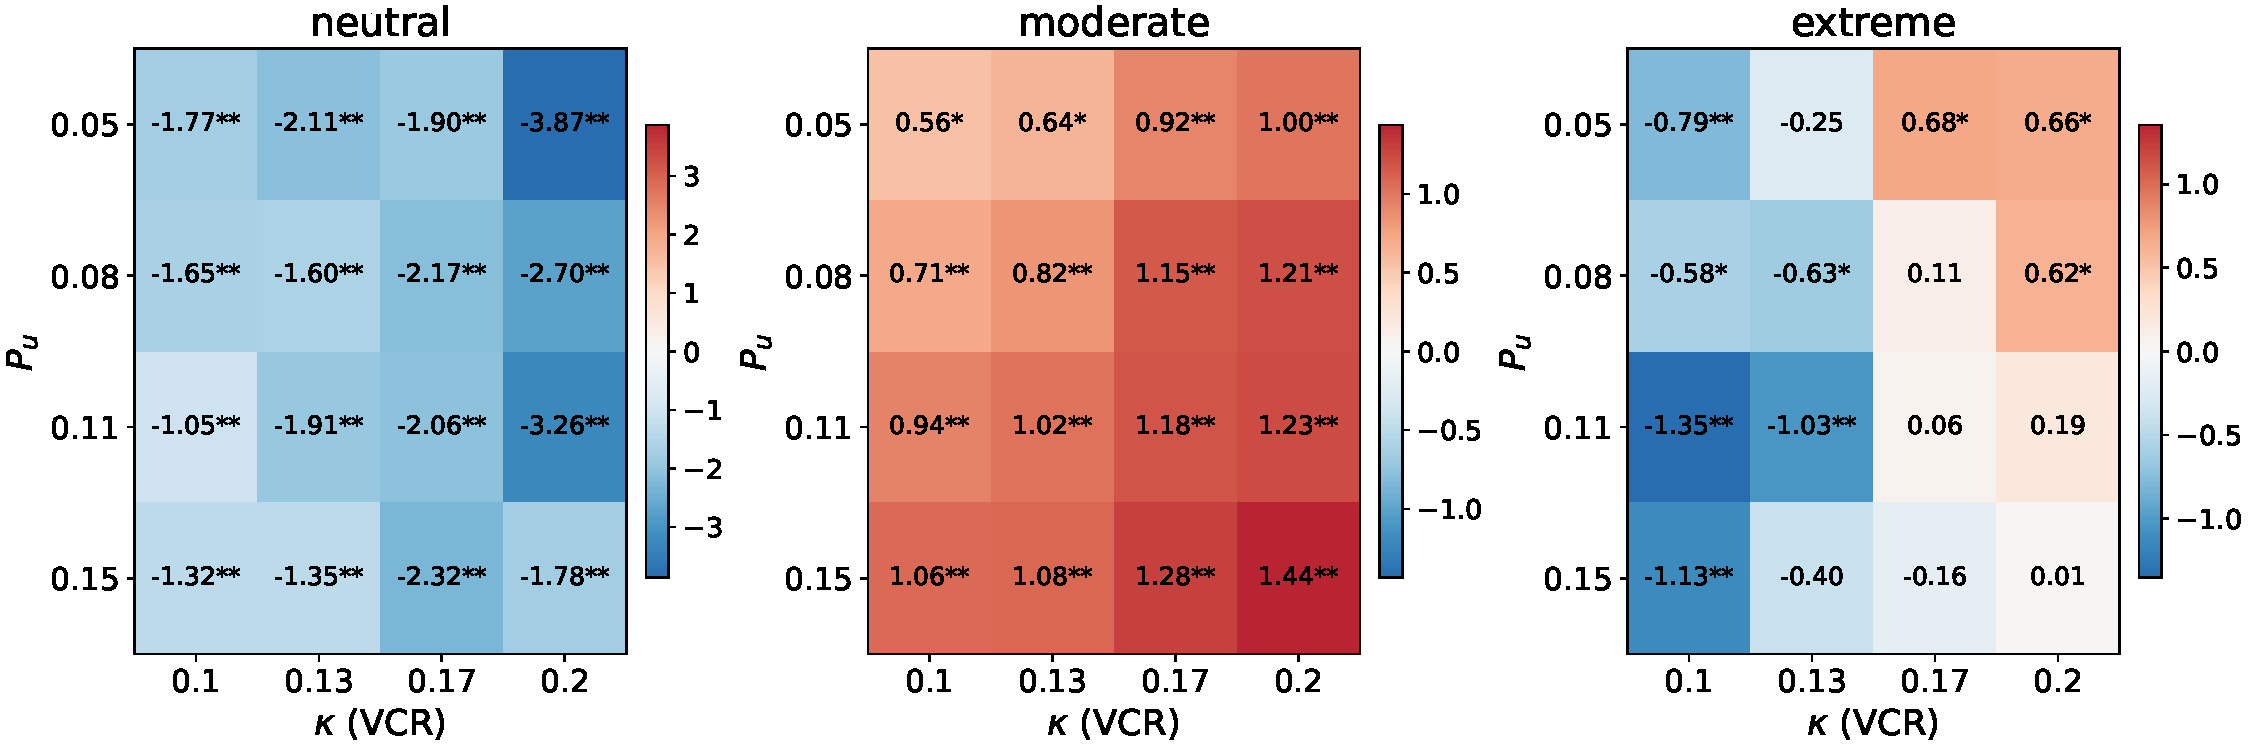
\includegraphics[width=\linewidth]{figures/outcome-heatmap.pdf}
\caption{Per-camp effect of neutral-hub silencing
on posting rate (N-silent -- control; paired Cohen's
$d_z$;\ignore{across seeds;}
one-sided paired $t$-test: $*$~$p<0.05$, $**$~$p<0.01$)}
\label{outcome-heatmap}
\end{figure}

\begin{figure}[t]
\centering
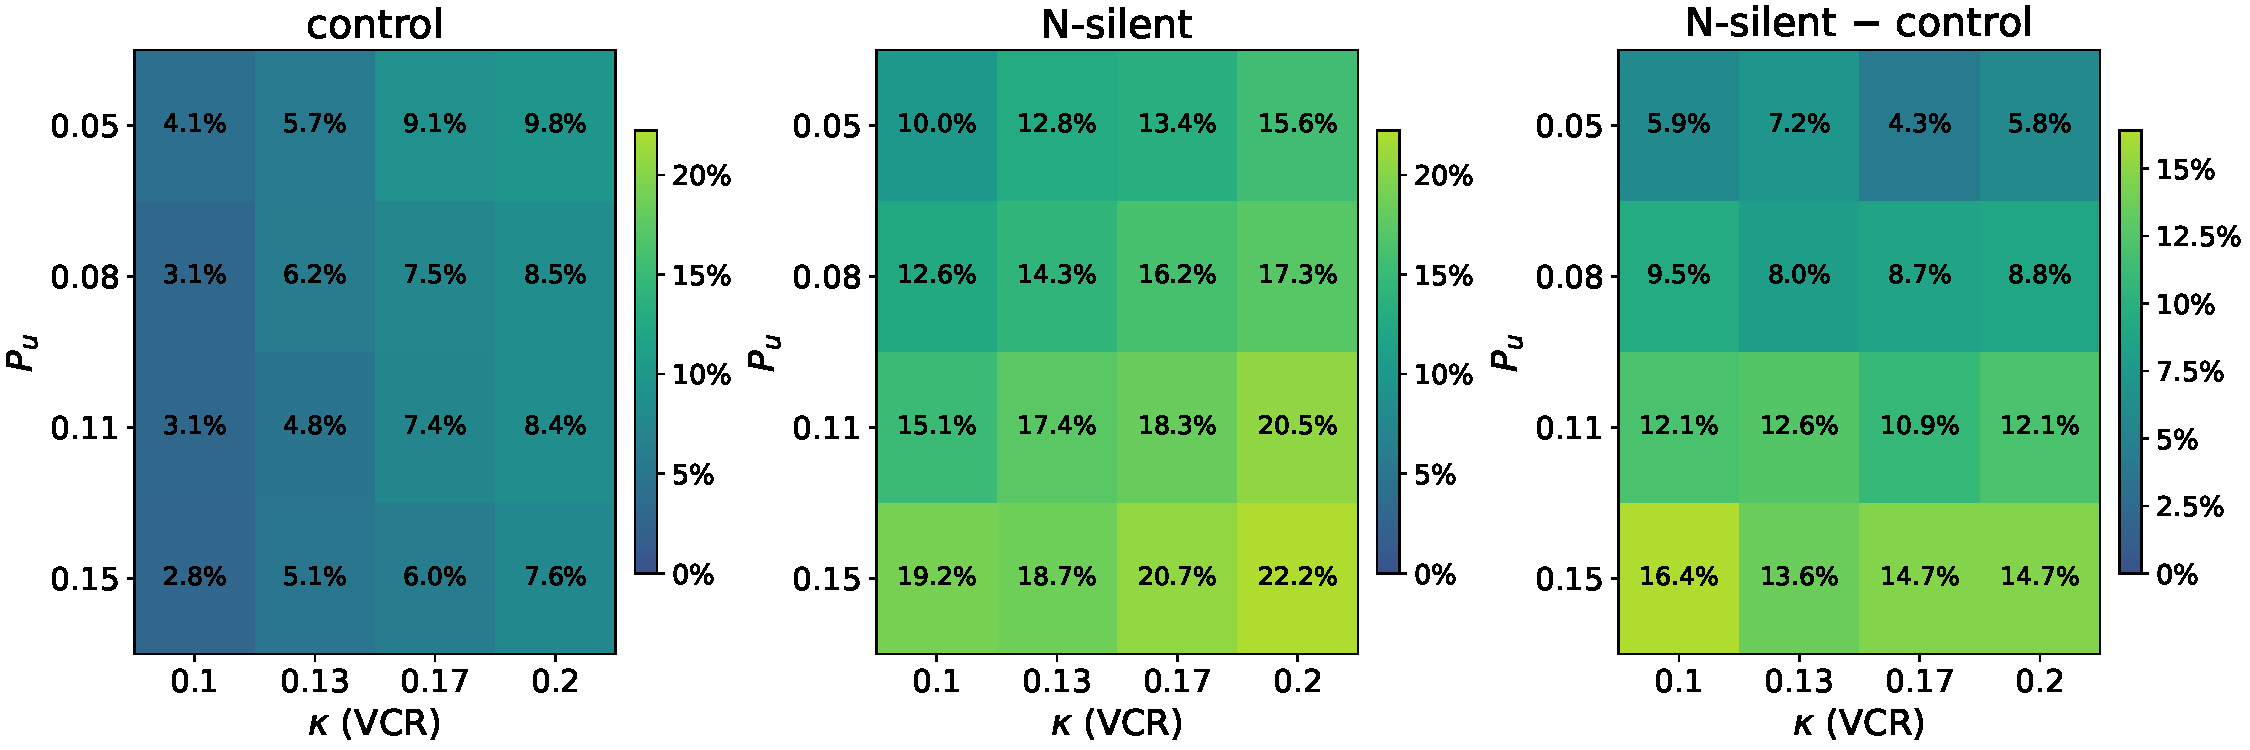
\includegraphics[width=\linewidth]{figures/mod-extreme-influx.pdf}
\caption{Late trailing-window share of an extreme agent's feed
occupied by same-signed moderate-authored content:
for \emph{control} and \emph{N-silent}
(left and center), and their difference (right).}
\label{mod-extreme-influx}
\end{figure}

\begin{figure}[t]
\centering
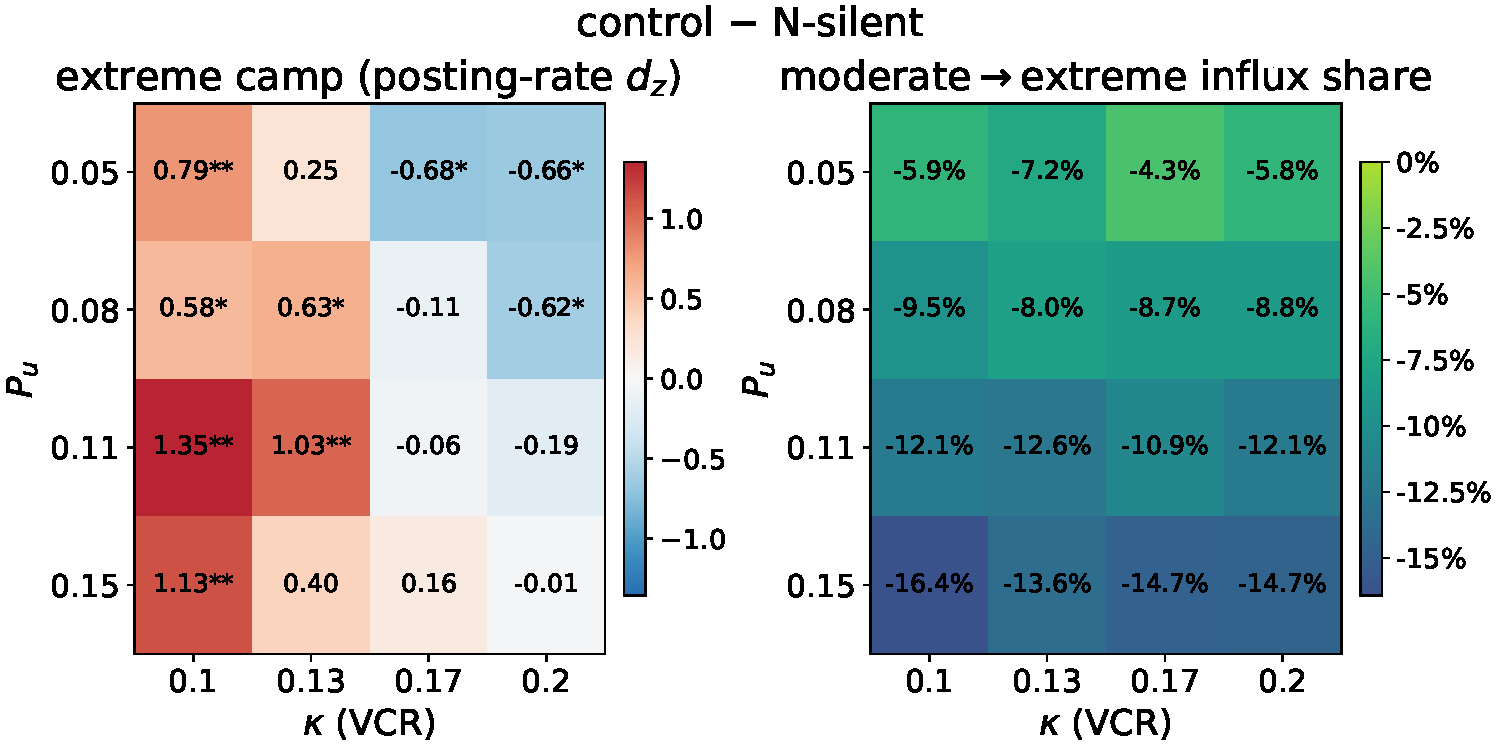
\includegraphics[width=0.8\linewidth]{figures/control-minus-msilent.pdf}
\caption{Same two complementary effects as Fig.~\ref{outcome-heatmap} right and
Fig.~\ref{mod-extreme-influx} right, with the contrast reversed to \emph{control}
$-$ \emph{N-silent}, framing them via the presence of an active
neutral hub: extreme-camp posting-rate effect size (left) and
moderate$\to$extreme influx share gap (right).}
\label{control-minus-msilent}
\end{figure}

\section{Experimental Results}\label{sec:results}
Fig.~\ref{outcome-heatmap} displays heatmaps of the paired Cohen's
$d_z$ (mean seed-wise difference divided by its standard deviation) in
per-capita posting rate across the three camps over the trailing
window $(38000, 40000]$, comparing \emph{N-silent} against
\emph{control} (\emph{N-silent}--\emph{control}). Neutrals
consistently increase posting activity when perceiving aligned hub
vocality, whereas moderates reduce theirs. In contrast, the
extreme camp exhibits a non-linear response: its posting is reduced
(negative $d_z$) at lower $\VCR$ values for each $P_u$ row, with the
sign-crossing point shifting across $P_u$ levels. Reversing the
contrast to \emph{control}--\emph{N-silent} frames these differences
via the presence of neutral hubs~(Fig.\ref{control-minus-msilent} left). From this perspective, for a given
$P_u$, neutral hubs facilitate extreme posting under low comfort
thresholds (low $\VCR$), and suppress it when higher nearby
agreement is required (high $\VCR$).
\par


Also, $P_u$ acts as a modulator that shifts the $\VCR$ sign-crossing
point, the watershed at which neutral-hub vocality switches between
facilitating and suppressing the extreme camp. In
Fig.~\ref{outcome-heatmap}, higher $P_u$ rows maintain negative effect
sizes over a broader low-$\VCR$ range before turning positive,
confirming that $P_u$ governs where this sign reversal occurs.
\par

To uncover the upstream mechanism behind the neutral hubs' cross-over
effect on extremes, we examine the interplay between moderates and
extremes. Fig.~\ref{mod-extreme-influx} displays the trailing-window share of
an extreme agent's feed occupied by same-signed moderate
content. This share is consistently larger in \emph{N-silent} than in
\emph{control}. As shown in the rightmost panel, this asymmetric
influx difference is mainly governed by $P_u$, growing several-fold as
$P_u$ increases, and only weakly by $\VCR$.
\par


\section{Discussion}\label{sec:discussion}
The sign-consistent responses of neutrals (suppressed) and moderates
(amplified) in Fig.~\ref{outcome-heatmap} follow from a single
mechanism: by construction (Eq.~\eqref{eq:social-reinforcement}), an
agent's posting probability depends solely on the comfortable fraction
$c_i(t)$ of its feed. Neutral hubs therefore directly move the posting
behavior of whichever camp receives their output in substantial
volume. For the neutral camp, hub opinions align with the neutral
range, placing almost every hub post within the agents' vocal comfort
radius $\VCR$; since neutral hubs supply the vast majority of
neutral-authored content, they occupy nearly $80\%$ of a neutral
agent's feed in control conditions. Silencing them removes this large
body of homophilic content, cutting the average feed-comfort fraction
from roughly $50\%$ to $30\%$ and driving posting down. For moderates,
by contrast, neutral hubs occupy $25\%\text{--}50\%$ of their feeds
(depending on $P_u$) in control conditions while falling almost entirely outside their
comfort range: active hubs dilute the moderates' comfort ratio and
suppress their posting, whereas silencing them removes this dilution and
reactivates them.
\par


The extreme camp's response, however, cannot be explained by these
direct mechanisms, as neutral-hub content occupies only a few percent
of an extreme agent's feed in all control conditions; its sign
reversal must therefore be a downstream ripple effect. We argue this
operates through two sequential layers: an \emph{openness} layer
(homophily-driven gating) that determines how opinion-distant the
content admitted into an extreme agent's feed can be, followed by a
\emph{comfort} layer (a spiral-of-silence mechanism) that determines
whether that arriving content is evaluated as supportive or
disruptive.
\par


The openness mechanism is governed by $P_u$ and operates via
$\BoundedConfidence_i(t)$. Since ties are formed or severed based on
this homophilic threshold, it determines whether a moderate author is
followed or blocked, and the gating is non-uniform: a narrow
$\BoundedConfidence_i(t)$ admits only the extreme-ward edge of
moderates, whereas a wider one extends admission toward their
neutral-ward edge. Higher $P_u$ correlates with a wider converged
$\BoundedConfidence_i(t)$ among extreme agents, a monotonic trend
observed across all $\VCR$ strata (Kendall's $\tau=0.29\text{--}0.38$,
$p<10^{-4}$): while $\BoundedConfidence_i(t)$ drops initially due to
exposure to out-of-tolerance content, a higher $P_u$ prunes distant
sources faster, allowing it to recover to a wider threshold. Higher
$P_u$ thus opens connection opportunities toward neutral-ward
moderates.
\par

Supporting this role of $P_u$, the condition gap in moderate post
volume reaching extreme feeds (Fig.~\ref{mod-extreme-influx}) grows
consistently with $P_u$, and the same holds at the graph level: the
\emph{N-silent}--\emph{control} gap in mean directed edges from
extreme to same-sign moderate agents at $t=40{,}000$ rises from
$+0.08$ at $P_u=0.05$ to $+0.22$ at $P_u=0.15$.
\par



The comfort mechanism, in contrast, is governed by $\VCR$. Whatever
moderate content the openness mechanism admits, $\VCR$ dictates
its evaluation: content within $\VCR$ is processed as comfortable,
while content outside it acts as disruptive. This evaluation role
fixes the direction of the extreme camp's sign reversal. Under a
narrow $\VCR$, little of the admitted moderate content falls
within the comfort range, diluting the comfort ratio and suppressing
posting; under a wide $\VCR$, a non-trivial share falls inside,
boosting posting instead. Thus, for a given $P_u$, silencing neutral
hubs suppresses extreme posting when $\VCR$ is low, but activates it
when $\VCR$ is high. As shown in Fig.~\ref{outcome-heatmap}, this
sign-crossing point shifts toward higher $\VCR$ as $P_u$ increases,
because the wider $\BoundedConfidence_i(t)$ admits more neutral-ward
moderate sources, requiring a wider $\VCR$ for their content to
register as comfortable.
\par


To capture the specific effect of an \emph{active} neutral hub, we
restate this mechanism from the perspective of activation rather than
silencing (Fig.~\ref{control-minus-msilent}). Its positive region is
the facilitating regime, where an active neutral hub
counterintuitively boosts extreme posting, and its negative region the
suppressing regime. Both follow from the moderate suppression
established above: by diluting the moderates' comfort ratio, an active
neutral hub deactivates the very source of the moderate content that
would otherwise reach extreme feeds under \emph{N-silent}. Under a
narrow $\VCR$ that content would have been disruptive, thereby withholding
it keeps the extreme camp's feed comfortable; under a wide $\VCR$ it
would have been comfortable, thereby withholding it deprives the camp of a
comfortable source. Which of the two regimes applies is set by
$\BoundedConfidence_i(t)$, the same openness threshold discussed
above: a higher $P_u$ widens $\BoundedConfidence_i(t)$ and thereby
extends admission toward the neutral-ward edge of moderates, then the
moderate content an active hub withholds grows more opinion-distant
from the extreme agent as $P_u$ increases. Since more opinion-distant
content requires a correspondingly wider $\VCR$ before it registers as
comfortable in the first place, the point at which withholding it
switches from removing a disruptive source to removing a comfortable
one shifts toward higher $\VCR$ as well. In this sense $P_u$ sets the
sign-crossing $\VCR$ indirectly, by governing how opinion-distant the
moderate content is that an active neutral hub keeps out of the
extreme camp's feed. An active neutral hub therefore operates less as
a passive conduit than as an upstream regulator of posting activity.

\section{Conclusion}\label{sec:conclusion}
In this study, we investigated how neutral-hub activity shapes
vocalization dynamics in an agent-based model on a heavy-tailed follow
network. Neutral hubs exert direct, opposing effects on neutral and
moderate populations: they amplify posting among aligned neutrals
while suppressing it among moderates. In contrast, their effect
on extreme agents is indirect and non-linear, driven by changes in
moderate content flows. This downstream effect operates through
two layered mechanisms: an \emph{openness} layer that gates
moderate content exposure, and a \emph{comfort} layer that
evaluates arriving content, causing the net effect on extreme posting
to reverse across parameter regimes. 
Rather than passive bridges
connecting distant camps, neutral hubs can act as upstream regulators
whose activity reshapes the broader information environment.

These findings should be interpreted within the assumptions of the
model. In particular, the observed sign reversal depends on the
interaction between adaptive exposure and 
comfort-driven posting, and
the model abstracts opinion into a single dimension while omitting
other features of social media, such as recommendation mechanisms 
and complex interaction with news media. 
The present results therefore do not imply
that neutral-hub activity will necessarily produce the same effects. 
Nevertheless, within this simplified setting, the observed 
patterns provide a meaningful indication that neutral-hub 
activity can generate indirect and counterintuitive 
downstream effects by reshaping vocality and 
information flows across the network.
Examining
whether similar mechanisms emerge under alternative network,
behavioral, and platform conditions, and validating these dynamics
against empirical data, remains an important direction for future
work.

%
\Black%%{}######
%

\bibliographystyle{spmpsci}
\bibliography{refs}
\end{document}
